\section{Introduction}
\label{sec:introduction}

\subsection{Human-Robot Search}
\label{subsec:cordon_and_search}

A search task focuses on walking through the search space to find target objects or persons of interest.
It has been included in many assignments, like military cordon and search \cite{waggener2010air}, wilderness search and rescue, and etc.  
The agents in a search team are usually required to collaborate to enhance the search efficiency.
The collaboration in a team search task involves information gathering and sharing in team wide of a multi-agent system.
Due to the capacity asymmetry between a robot agent and a human agent, adding a robot to a search team facilitate the team capability. 
The advantages of involving robots in a search team potentially include follows:
\begin{enumerate}
\item robots can be assigned some tasks to reduce potential danger to humans;
\item robots can deliver constant and stable performance without fatigue; 
\item robots can be equipped with a variety of sensors that can extend the perception capability of the entire team.
\end{enumerate}

\subsection{Robot Wingman}
\label{subsec:robot_wingman}

To support the collaboration in the search task, \cite{goodrich2013toward} introduce a robot wingman. 
The robot wingman defines a type of human-robot relationship in a team, which is to have a robot that accompanies a human when the human navigates through some space.
Besides the advantages from a robot agent in a search team, a robot wingman can also
\begin{enumerate}
\item detect threats or opportunities that may be relevant to the human but likely not seen by the human;
\item be responsive to an assistance request from a human agent in the team. 
\end{enumerate}

\begin{figure}[htbp]
\centering
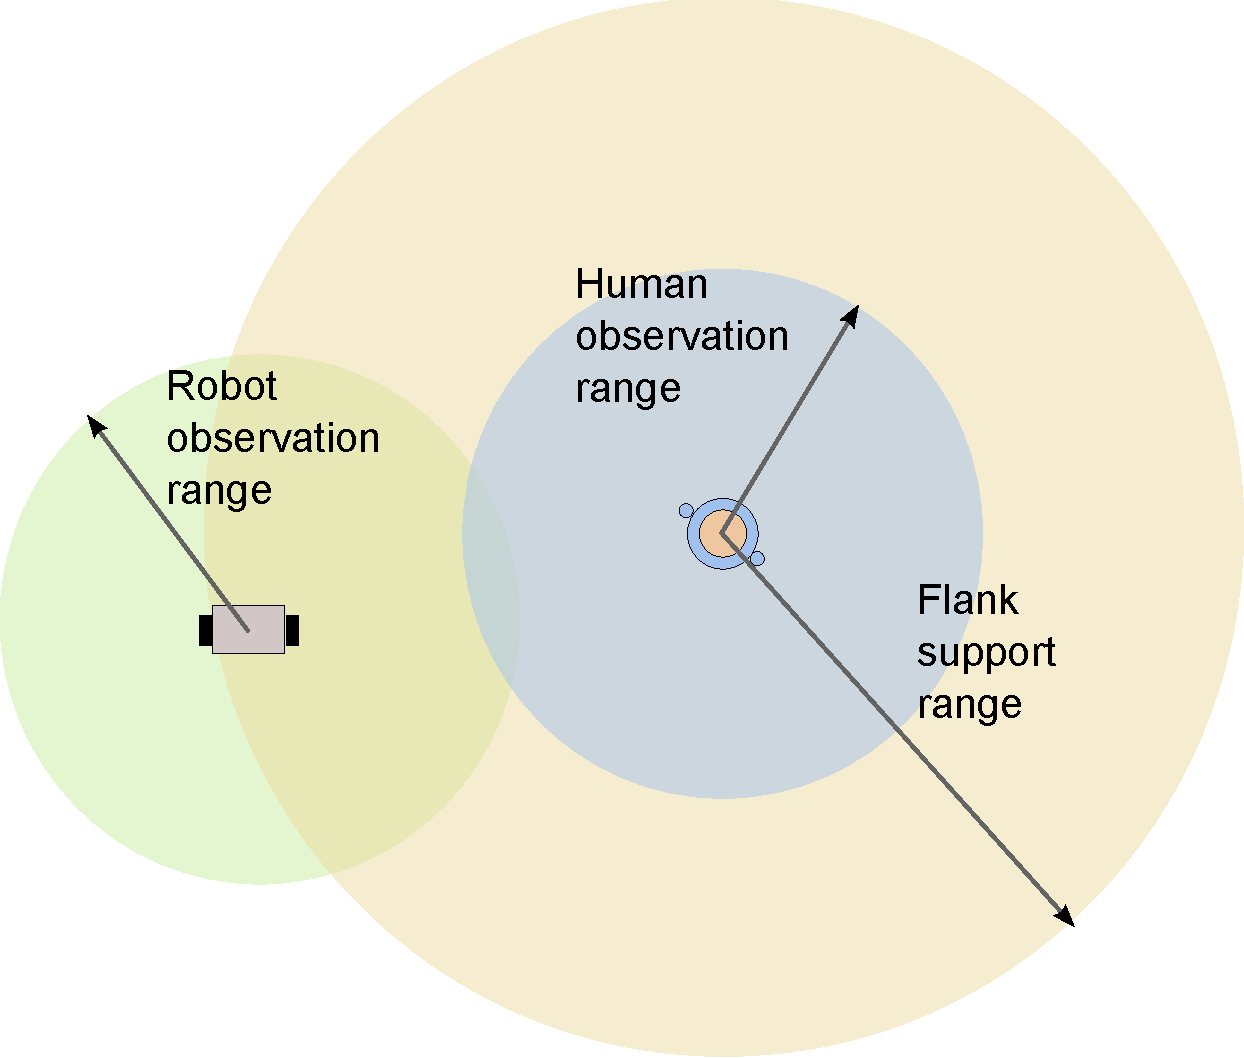
\includegraphics[width=0.4\textwidth]{./images/Wingman.pdf}
\caption{A Robot Wingman Framework.}
\label{fig:Wingman}
\end{figure}

The paper proceeds as follows.
We give a brief review on how the model is usually modeled and how the problems are solved in Section \ref{sec:related_work}.
Section \ref{sec:problem_statement} gives how the problem is modeled into an information maximization problem and how a multi-partite graph is generated using the wingman constraint.
Section \ref{sec:path_dependent_optimization} formulates the problem into a class of submodular orienteering on a multi-partite graph.
Section \ref{sec:tree_expanding_search} proposes the algorithms on solving the submodular orienteering and provides the proof on the  performance.
Section \ref{sec:simulation_and_analysis} analyzes the performance and efficiency of the proposed algorithm in different scenarios and parameters.
